        \documentclass{standalone}
        \usepackage{tikz}
        \begin{document}
        \fontsize{16px}{16px}\selectfont
        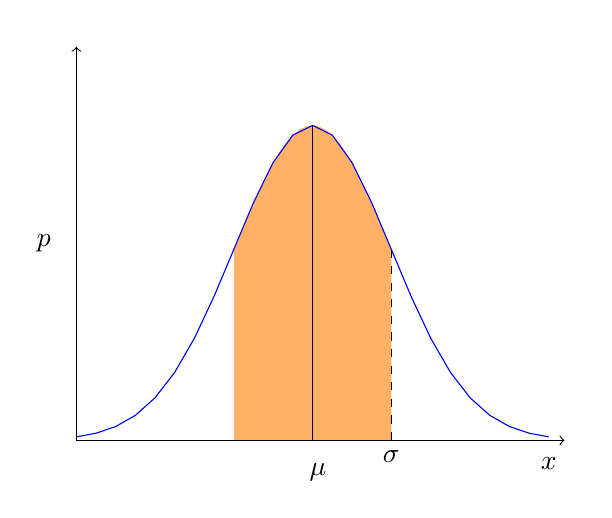
\begin{tikzpicture}


% define normal distribution function 'normaltwo'
    \def\normaltwo{\x,{4*1/exp(((\x-3)^2)/2)}}
 
% input y parameter
    \def\y{4}
 
% this line calculates f(y)
    \def\fy{4*1/exp(((\y-3)^2)/2)}
 
% Shade orange area underneath curve.
    \fill [fill=orange!60] (2,0) -- plot[domain=2:4] (\normaltwo) -- ({\y},0) -- cycle;
 
% Draw and label normal distribution function
    \draw[color=blue,domain=0:6] plot (\normaltwo) node[right] {};
 
% Add dashed line dropping down from normal.
    \draw[dashed] ({\y},{\fy}) -- ({\y},0) node[below] {$\sigma$};
 
% Optional: Add axis labels
    \draw (-.2,2.5) node[left] {$p$};
    \draw (6,-.1) node[below] {$x$};
    \draw (3,0) -- (3, 4);
    \draw (3.3,-0.4) node[left] {$\mu$};
 
% Optional: Add axes
    \draw[->] (0,0) -- (6.2,0) node[right] {};
    \draw[->] (0,0) -- (0,5) node[above] {};
        \end{tikzpicture}
        \end{document}
